
\documentclass[a4paper,11pt]{article}
\usepackage[a4paper, margin=8em]{geometry}

% usa i pacchetti per la scrittura in italiano
\usepackage[french,italian]{babel}
\usepackage[T1]{fontenc}
\usepackage[utf8]{inputenc}
\frenchspacing 

% usa i pacchetti per la formattazione matematica
\usepackage{amsmath, amssymb, amsthm, amsfonts}

% usa altri pacchetti
\usepackage{gensymb}
\usepackage{hyperref}
\usepackage{standalone}

% imposta il titolo
\title{Appunti Comunicazioni Numeriche}
\author{Luca Seggiani}
\date{2026}

% imposta lo stile
% usa helvetica
\usepackage[scaled]{helvet}
% usa palatino
\usepackage{palatino}
% usa un font monospazio guardabile
\usepackage{lmodern}

\renewcommand{\rmdefault}{ppl}
\renewcommand{\sfdefault}{phv}
\renewcommand{\ttdefault}{lmtt}

% disponi il titolo
\makeatletter
\renewcommand{\maketitle} {
	\begin{center} 
		\begin{minipage}[t]{.8\textwidth}
			\textsf{\huge\bfseries \@title} 
		\end{minipage}%
		\begin{minipage}[t]{.2\textwidth}
			\raggedleft \vspace{-1.65em}
			\textsf{\small \@author} \vfill
			\textsf{\small \@date}
		\end{minipage}
		\par
	\end{center}

	\thispagestyle{empty}
	\pagestyle{fancy}
}
\makeatother

% disponi teoremi
\usepackage{tcolorbox}
\newtcolorbox[auto counter, number within=section]{theorem}[2][]{%
	colback=blue!10, 
	colframe=blue!40!black, 
	sharp corners=northwest,
	fonttitle=\sffamily\bfseries, 
	title=~\thetcbcounter: #2, 
	#1
}

% disponi definizioni
\newtcolorbox[auto counter, number within=section]{definition}[2][]{%
	colback=red!10,
	colframe=red!40!black,
	sharp corners=northwest,
	fonttitle=\sffamily\bfseries,
	title=~\thetcbcounter: #2,
	#1
}

% U.D.M
\newcommand{\amp}{\ensuremath{\mathrm{A}}}
\newcommand{\volt}{\ensuremath{\mathrm{V}}}
\newcommand{\meter}{\ensuremath{\mathrm{m}}}
\newcommand{\second}{\ensuremath{\mathrm{s}}}
\newcommand{\farad}{\ensuremath{\mathrm{F}}}
\newcommand{\henry}{\ensuremath{\mathrm{H}}}
\newcommand{\siemens}{\ensuremath{\mathrm{S}}}

% circuiti
\usepackage{circuitikz}
\usetikzlibrary{babel}

% disegni
\usepackage{pgfplots}
\pgfplotsset{width=10cm,compat=1.9}

% disponi codice
\usepackage{listings}
\usepackage[table]{xcolor}

\lstdefinestyle{codestyle}{
		backgroundcolor=\color{black!5}, 
		commentstyle=\color{codegreen},
		keywordstyle=\bfseries\color{magenta},
		numberstyle=\sffamily\tiny\color{black!60},
		stringstyle=\color{green!50!black},
		basicstyle=\ttfamily\footnotesize,
		breakatwhitespace=false,         
		breaklines=true,                 
		captionpos=b,                    
		keepspaces=true,                 
		numbers=left,                    
		numbersep=5pt,                  
		showspaces=false,                
		showstringspaces=false,
		showtabs=false,                  
		tabsize=2
}

\lstdefinestyle{shellstyle}{
		backgroundcolor=\color{black!5}, 
		basicstyle=\ttfamily\footnotesize\color{black}, 
		commentstyle=\color{black}, 
		keywordstyle=\color{black},
		numberstyle=\color{black!5},
		stringstyle=\color{black}, 
		showspaces=false,
		showstringspaces=false, 
		showtabs=false, 
		tabsize=2, 
		numbers=none, 
		breaklines=true
}

\lstdefinelanguage{javascript}{
	keywords={typeof, new, true, false, catch, function, return, null, catch, switch, var, if, in, while, do, else, case, break},
	keywordstyle=\color{blue}\bfseries,
	ndkeywords={class, export, boolean, throw, implements, import, this},
	ndkeywordstyle=\color{darkgray}\bfseries,
	identifierstyle=\color{black},
	sensitive=false,
	comment=[l]{//},
	morecomment=[s]{/*}{*/},
	commentstyle=\color{purple}\ttfamily,
	stringstyle=\color{red}\ttfamily,
	morestring=[b]',
	morestring=[b]"
}

% disponi sezioni
\usepackage{titlesec}

\titleformat{\section}
	{\sffamily\Large\bfseries} 
	{\thesection}{1em}{} 
\titleformat{\subsection}
	{\sffamily\large\bfseries}   
	{\thesubsection}{1em}{} 
\titleformat{\subsubsection}
	{\sffamily\normalsize\bfseries} 
	{\thesubsubsection}{1em}{}

% disponi alberi
\usepackage{forest}

\forestset{
	rectstyle/.style={
		for tree={rectangle,draw,font=\large\sffamily}
	},
	roundstyle/.style={
		for tree={circle,draw,font=\large}
	}
}

% disponi algoritmi
\usepackage{algorithm}
\usepackage{algorithmic}
\makeatletter
\renewcommand{\ALG@name}{Algoritmo}
\makeatother

% disponi numeri di pagina
\usepackage{fancyhdr}
\fancyhf{} 
\fancyfoot[L]{\sffamily{\thepage}}

\makeatletter
\fancyhead[L]{\raisebox{1ex}[0pt][0pt]{\sffamily{\@title \ \@date}}} 
\fancyhead[R]{\raisebox{1ex}[0pt][0pt]{\sffamily{\@author}}}
\makeatother

\begin{document}
% sezione data)
\section{Lezione del 05-03-26}

% stili pagina
\thispagestyle{empty}
\pagestyle{fancy}

% testo
\subsection{Introduzione ai processi aleatori}
Veniamo alla parte del corso dove trattiamo di:
\begin{itemize}
	\item Elementi di probabilità;
	\item Variabili aleatorie;
	\item Processi stocastici.
\end{itemize}

Questa parte di teoria ci sarà utile nel caso di processi che si evolvono nel tempo in maniera \textit{non deterministica}, o meglio \textbf{aleatoria}. Dal punto di vista matematico, avremo bisogno di partire dalle basi della teoria della \textbf{probabilità}.

Un modello si definisce \textit{deterministico} se non vi è alcuna incertezza riguardo il suo comportamento ad ogni istante di temo. Ad esempio, i sistemi lineari tempo-invariante (\textbf{LTI}, si rimanda agli appunti di automatica) sono sistemi deterministici, poiché i valori delle loro uscite possono essere completamente determinati a priori noti i valori dei loro ingressi.

In molte situazioni reali (fra cui quelle che studieremo nel campo delle comunicazioni digitali) i modelli deterministici sono inappropiati e necessitiamo di un modello che tenga conto di molti valori sconosciuti. In questo caso dobbiamo trovare uno strumento matematico per modellare l'\textit{incertezza}.

\subsubsection{Modelli probabilistici}
I \textbf{modelli probabilistici} sono necessari per progettare sistemi che:
\begin{itemize}
	\item Rispondono a forte incertezza;
	\item Sono computazionalmente efficienti;
	\item E sono economicamente convenienti.
\end{itemize}

Prendiamo l'esempio di un sistema di comunicazione digitale su un canale \textit{wireless}:
\begin{center}
	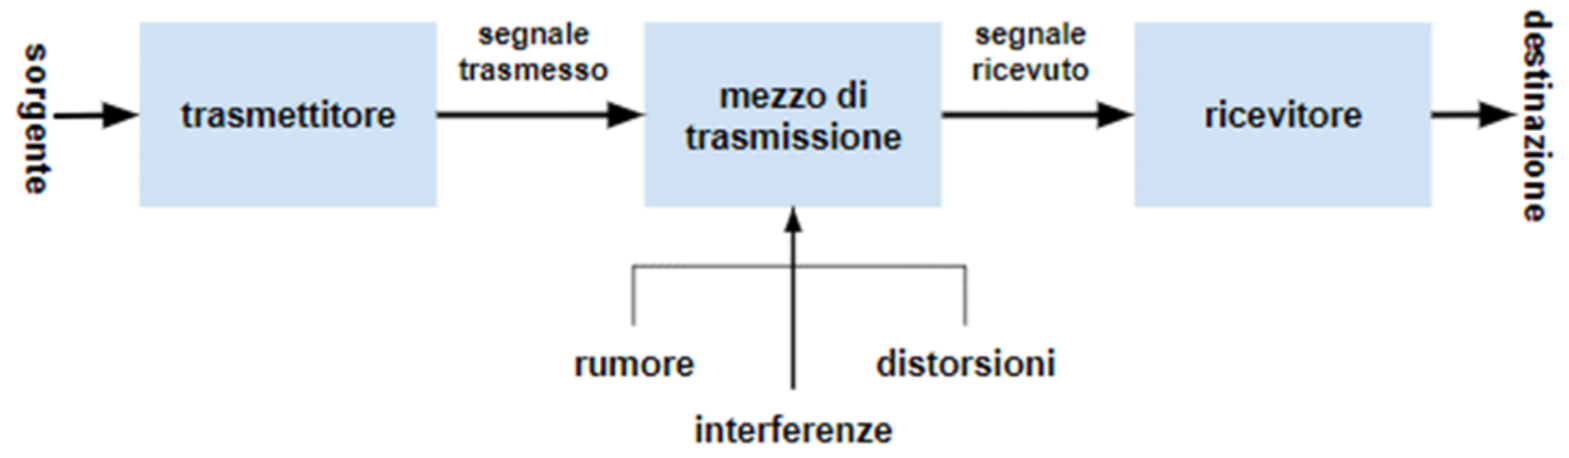
\includegraphics[scale=0.3]{../figures/wifi_prob.png}
\end{center}

Come vediamo, abbiamo diversi elementi di natura aleatoria, fra cui:
\begin{itemize}
	\item Il \textbf{rumore} di fondo del mezzo;
	\item Le \textbf{interferenze} da parte di altri trasmettitori;
	\item Le \textbf{distorsioni} date dalla natura del mezzo (ad esempio il fading del canale).
\end{itemize}
Il segnale ricostruito al ricevitore è quindi tipicamente una replica attenuata del segnale trasmesso più un contenuto di disturbo, ed è quindi modellabile come un \textit{processo aleatorio}.

Un'altro campo in cui la modellazione aleatoria è particolarmente utile è quello di componenti che hanno una certà possibilità di \textit{"fallire"}. In questo caso, ci forniscono uno strumento matematicamente accurato per valutare la tolleranza dei sistemi costituiti da tali componenti.

Vediamo un ultimo esempio. Preso un protocollo di \textbf{MAC} (\textit{Medium Access Control}) come ALOHA slotted, dove il tempo è diviso in slot, potremmo trovare una situazione simile:
\begin{center}
	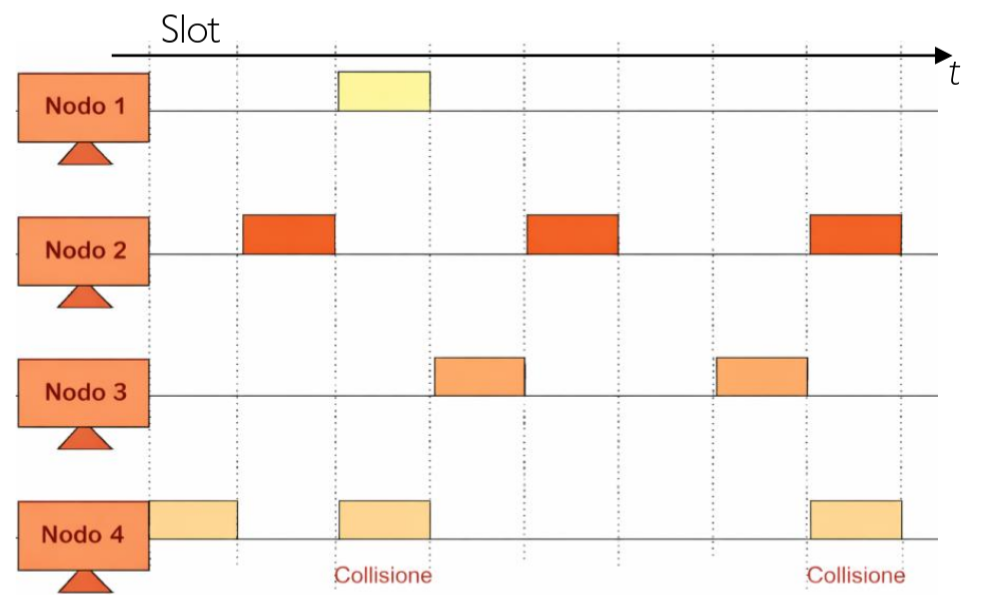
\includegraphics[scale=0.4]{../figures/aloha_prob.png}
\end{center}
dove ogni nodo (fra $N$ nodi totali) trasmette ad ogni slot temporale con probabilità $p$. In questo caso i modelli probabilistici possono aiutarci a calcolare la probabilità di successo per la trasmissione di uno o di tutti i nodi in un dato slot (chiamiamola $p_s$), e di determinare il valore ottimo di $p$ (chiamiamolo $p^*$) che massimizza $p_s$. 
Notiamo che calcoli di questo tipo sono stati già fatti negli appunti a \url{https://seggiani-luca.github.io/appunti-cn/master.pdf}, nei capitoli su ALOHA e ALOHA slotted.

Prendiamo quindi la probabilità che un singolo nodo trasmetta con successo in un dato slot come:
$$
p(1-p)^N-1 \implies p_s = N p(1-p)^N-1 
$$
da cui si ricava subito la probabilità che una trasmissione efficace avvenga fra tutti i nodi.

Sia $p_s$ una funzione di $p$, e $N = 10$, cioè:
$$
p_s(p, N) = N p(1-p)^N-1, \quad p \in [0, 1], \ N = 10
$$
Potremmo tracciare tale funzione su un grafico come:
\begin{center}
	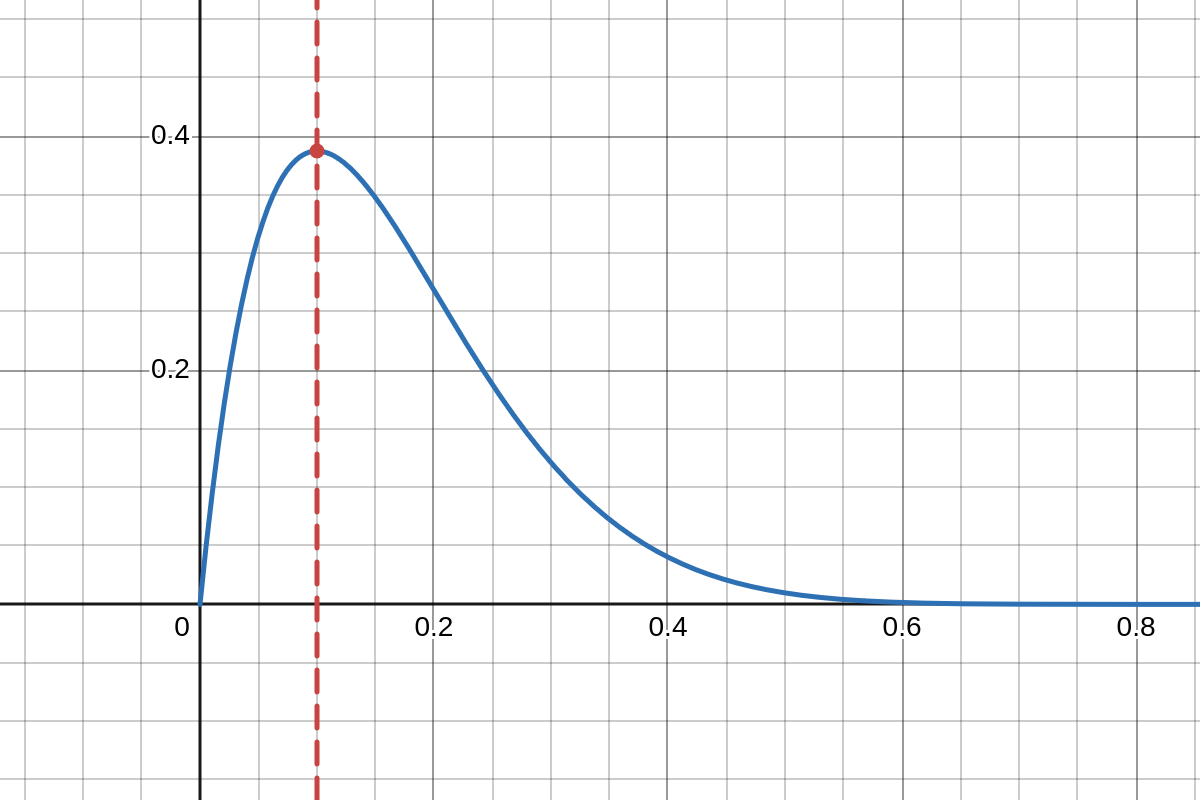
\includegraphics[scale=0.28]{../figures/aloha_max.png}
\end{center}
dove si evidenziato il valore ottimo $p^*$ di probabilità di trasmissione. Attraverso la derivazione nel documento allegato prima, o anche solo per intuizione, arriviamo alla conclusione che:
$$
p^* = \frac{1}{N} = = 0.1
$$
cioè la probabilità ottima è uno sul numero di utenti che trasmettono sulla rete. Sostituendo questo valore di $p$ in $p_s$, possiamo tracciare la funzione al variare degli utenti $N$, cioè:
$$
p_s(p, N) = N p(1-p)^N-1, \quad p = p^* = \frac{1}{N}, N \in \mathbb{N} \implies p_s(N) = (1 - \frac{1}{N})^N
$$
quseta funzione è nota e di limite immediato immaginando infiniti dispositivi (il caso peggiore):
$$
\lim_{N \rightarrow \infty} p_s(N) = \lim_{N \rightarrow \infty} (1 - \frac{1}{N})^N = \frac{1}{e}
$$

\newpage

Possiamo tracciarla su un grafico per essere sicuri della derivazione:
\begin{center}
	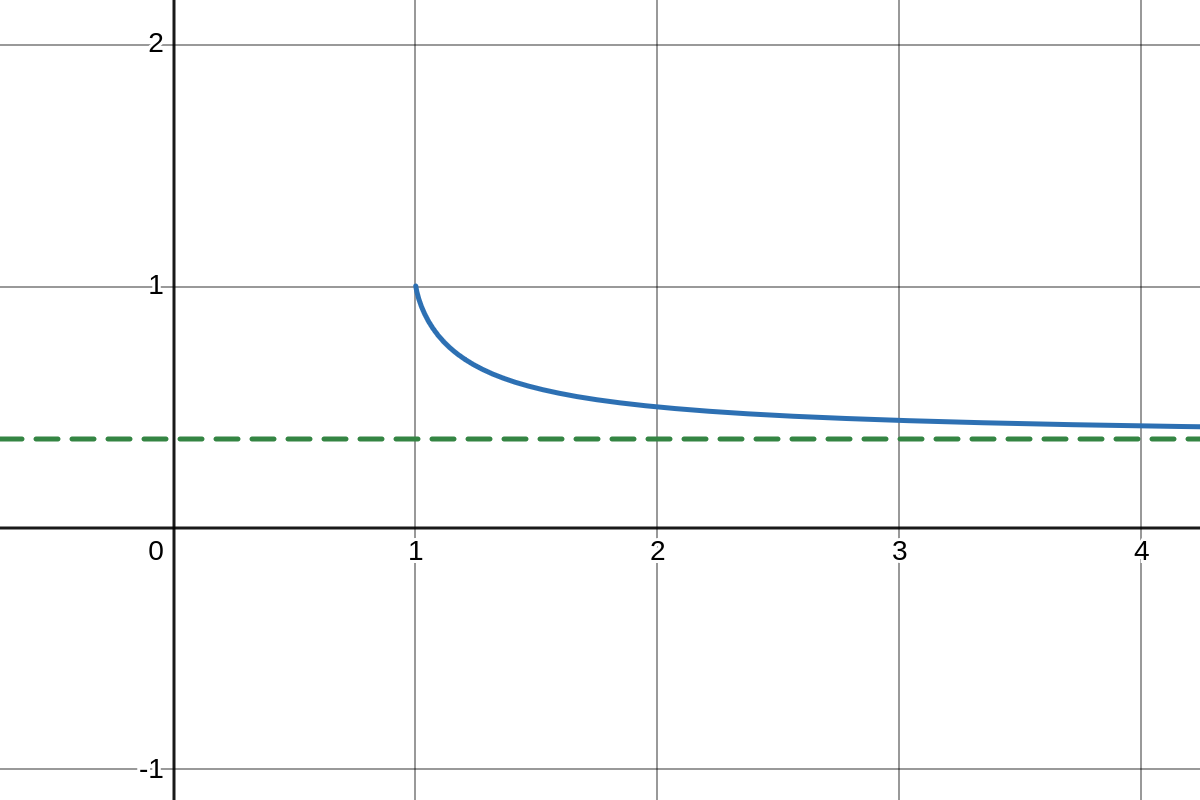
\includegraphics[scale=0.28]{../figures/aloha_limit.png}
\end{center}
da dove si vede chiaramente che il ramo di funzione tende al valore $\frac{1}{e} \approx 0.37$.

Abbiamo quindi trovato un problema legato al mondo delle comunicazioni numeriche, che teorie di tipo probabilistico riescono a descrivere, e attraverso le quali riusciamo ad avere buone stime dell'efficienza nel caso peggiore di operazione 

\subsubsection{Trattazione matematica}
La teoria della probabilità ha come obiettivo:
\begin{itemize}
	\item La descrizione matematica dei modelli probabilistici;
	\item Lo sviluppo di procedure di ragionamento che tengano traccia dell'incertezza.
\end{itemize}

\par\smallskip

\noindent
\textbf{\textsf{Teoria degli insiemi}}

\noindent
Cominciamo da richiami sulla teoria degli \textbf{insiemi}.
Un insieme $A = \{ x, y, ... \}$ è una \textit{collezione} di oggetti, i cui elementi vengono detti \textit{elementi} $x \in A$. Gli elementi che \textit{non} appartengono ad un insieme si notano come $z \notin A$.
Indichiamo con $\emptyset$ l'insieme vuoto.
Notiamo che si possono indicare gli insiemi anche per proprietà comune: 
$$ 
[0, 1 = \{ x: 0 \leq x < 1 \}, \quad ...
$$ 

Sugli insiemi sono definite le classiche operazioni $\cup$, $\cap$, $\setminus$, (unione, intersezione, differenza), e le relazioni $\subset$, $\subseteq$ (sottoinsieme stretto, sottoinsieme), ecc... Ricordiamo la proprietà:
$$
\{ A \cap B \} \subset \{ A \cup B \}
$$

Un insieme che ci risulterà particolarmente utile è l'insieme $\Omega$, cioè lo spazio delle \textbf{possibilità}, detto anche spazio \textit{campione}.
Abbiamo che il numero possibile di sottoinsiemi di $\Omega$, se $\Omega$ ha $N$ elementi, è $2^N$.

Noto uno spazio campione $\Omega$, abbiamo a disposizione l'operazione di \textbf{complemento}, per cui possiamo dire $\bar{\emptyset} = \Omega$, $\bar{\Omega} = \emptyset$, e così via.

Diciamo quindi due insiemi \textit{disgiunti} se vale:
$$
A \cap B = \emptyset \implies \text{A e B sono disgiunti}
$$

Un insieme di insiemi disgiunti la cui unione dà un insieme $A$ viene detto partizione di $A$. In particolare:
$$
\mathcal{P}(A) = \{ a_1, a_2, ... \} \ \text{t.c.} \ \bigcup_i a_i = A
$$

Ricordiamo quindi alcune leggi fondamentali sull'algebra degli insiemi:

\begin{table}[H]
\centering
\renewcommand{\arraystretch}{1.5}
\begin{tabular}{lll}
\multicolumn{3}{c}{\textbf{Leggi di idempotenza}} \\ \hline
1a. & $A \cup A = A$ & 1b. $A \cap A = A$ \\ 

\multicolumn{3}{c}{\textbf{Leggi associative}} \\ \hline
2a. & $(A \cup B) \cup C = A \cup (B \cup C)$ & 2b. $(A \cap B) \cap C = A \cap (B \cap C)$ \\ 

\multicolumn{3}{c}{\textbf{Leggi commutative}} \\ \hline
3a. & $A \cup B = B \cup A$ & 3b. $A \cap B = B \cap A$ \\ 

\multicolumn{3}{c}{\textbf{Leggi distributive}} \\ \hline
4a. & $A \cup (B \cap C) = (A \cup B) \cap (A \cup C)$ & 4b. $A \cap (B \cup C) = (A \cap B) \cup (A \cap C)$ \\ 

\multicolumn{3}{c}{\textbf{Leggi di identità}} \\ \hline
5a. & $A \cup \emptyset = A$ & 5b. $A \cap U = A$ \\ 
6a. & $A \cup U = U$ & 6b. $A \cap \emptyset = \emptyset$ \\ 

\multicolumn{3}{c}{\textbf{Leggi di complementarietà}} \\ \hline
7a. & $A \cup A^c = U$ & 7b. $A \cap A^c = \emptyset$ \\ 
8a. & $(A^c)^c = A$ & 8b. $U^c = \emptyset$, $\emptyset^c = U$ \\ 

\multicolumn{3}{c}{\textbf{Leggi di De Morgan}} \\ \hline
9a. & $(A \cup B)^c = A^c \cap B^c$ & 9b. $(A \cap B)^c = A^c \cup B^c$ \\ 

\end{tabular}
\end{table}

\par\smallskip

\noindent
\textbf{\textsf{Teoria della probabilità}}

\noindent
La teoria della \textbf{probabilità}, come abbiamo detto, ha lo scopo di descrivere fenomeni che non manifestano regolarità deterministica. Ciò che sfruttiamo è l'analisi \textit{a posteriori} degli eventi misurati, con l'obiettivo di estrarre un qualche tipo di \textit{regolarità globale}.

Chiamiamo quindi esperimento \textit{casuale} o \textit{aleatorio} il procedimento di osservazione dello stato finale del sistema (detto \textbf{risultato}). L'esperimento deve essere \textit{ripetibile}, indeterminate volte, secondo le stesse modalità.

Da qui la prima definizione importante di questo argomento:
\begin{definition}{Spazio campione}
	Viene detto \textbf{spazio campione} $\Omega$ è l'insieme di tutti i possibili risultati di un esperimento.
\end{definition}

Un \textbf{evento} è un sottoinsieme dello spazio campione. Quindi è un insieme di risultati individuabile da una data caratteristica comune. Diciamo:
\begin{itemize}
	\item Evento \textbf{certo}: lo spazio campione $\Omega$. Questo si verifica ad ogni prova;
	\item Evento \textbf{impossibile}: l'insieme vuoto $\emptyset$. Questo non si verifica per nessuna prova;
	\item Evento \textbf{elementare} $\alpha$, un solo elemento di $\Omega$, cioè il risultato di un esperimento.
\end{itemize}

In soldoni, lanciare un dado è l'esperimento, ottenere 4 è il risultato, e ottenere una faccia pari o dispari è l'evento.
Una prova è una singola esecuzione dell'esperimento in cui si ottiene l'evento $\alpha$ (cioè il risultato che $\alpha$ individua).

Usare la notazione insiemistica per definire gli eventi ci permette di applicare l'algebra degli insiemi agli eventi stessi.

\par\smallskip

\noindent
\textbf{\textsf{Concetto di probabilità}}

\noindent
Chiamiamo \textbf{probabilità} una funzione sul dominio degli eventi che restituisce la valutazione quantitativa della \textit{possibilità} che quell'evento si verifichi.
In simboli:
$$
P(a) \rightarrow [0, 1], \quad \text{con $a$ evento}
$$

Come vediamo, il codominio della probabilità è $[0, 1]$. Valori di $P(a)$ prossimi a $0$ rappresentano scarse possibilità che quell'evento si verifichi, mentre valori di $P(a)$ prossimi a $1$ rappresentano ottime probabilità che quell'evento si verifichi.

La definizione classica della probabilità è la seguente:
\begin{definition}{Definizione classica di probabilità}
	Dato uno spazio campione $\Omega$ di dimensione $M$, e sia $m_a$ il numero di elementi parte dell'evento $a$ in $\Omega$. In tal caso la probabilità dell'evento $a$ sarà:
	$$
		P(a) = \frac{m_a}{M}
	$$
\end{definition}

I vantaggi di questa definizione sono che:
\begin{itemize}
	\item Definisce la probabilità in maniera \textit{apropristica}, senza ricorrere a prove sperimentali;
\end{itemize}
Gli svantaggi sono che:
\begin{itemize}
	\item Si assume che tutti i risultati siano \textit{equiprobabili};
	\item Non si possono gestire i casi in cui i risultati non sono \textit{equiprobabili} (ad esempio un mazzo truccato).
\end{itemize}

Per risolvere questi problemi si è affermata una seconda definizione di probabilità:
\begin{definition}{Definizione frequentistica di probabilità}
	Si fa la definizione preventiva di \textbf{frequenza relativa} attinente l'evento $a$, che su $N$ prove è:
	$$
		f_N(a) = \frac{n_a}{N}
	$$
	\tcblower
	La probabilità dell'evento $A$ è quindi definita come limite:
	$$
	P(a) = \lim_{N \rightarrow \infty} f_N(a) = \lim_{N \rightarrow \infty} \frac{n_a}{N} 
	$$
\end{definition}

I vantaggi di questa definizione sono che:
\begin{itemize}
	\item Non si basa su ipotesi a propri ma sulla conoscenza a posteriori di un dato ottenuta attraverso prove;
	\item Definisce la probabilità anche se i possibili risultati non sono \textit{equiprobabili}; 
\end{itemize}
Gli svantaggi sono che:
\begin{itemize}
	\item Da un punto di vista matematico, il limite non si può valutare analiticamente;
	\item Da un punto di vista pratico, non sempre si possono avere un numero arbitrariamente grande di osservazioni. 
\end{itemize}

Dai limiti del modello \textbf{induttivo}, basato sull’interpretazione frequentista della probabilità, deriva l’opportunità di ricorrere al modello \textbf{deduttivo} dovuto a \textit{Kolmogorov}. Questa è una definizione di tipo assiomatico. In questo non dà una definizione diretta della probabilità 
ma accetta qualunque approccio, purché questo rispetti le proprietà fondamentali, assunte come assiomi; da questi con l’ausilio della logica e della matematica si deducono le altre proprietà come teoremi.

\begin{definition}{Definizione assiomatica della probabilità}
Basiamoci sulla definizione data inizialmente del concetto di probabilità, cioè quello di una funzione:
$$
P(a) \rightarrow [0, 1], \quad \text{con $a$ evento}
$$

\tcblower

Diamo quindi i 3 assiomi di \textit{Kolmogorov}:
\begin{itemize}
	\item \textbf{Normalizzazione}: la probabilità dell'intero spazio campione $\Omega$ (quindi dell'evento \textit{certo}) dovrà essere uguale a $1$:
		$$
			P(\Omega) = 1
		$$
	\item \textbf{Non negatività}: la probabilità di un elemento dovrà essere un numero non negativo, per ogni evento $a$:
		$$
			P(a) \geq 0, \forall a
		$$
	\item \textbf{Additività}: se $a$ e $b$ sono 2 eventi disgiunti, allora dovrà essere soddisfatta l'uguaglianza:
		$$
			P(a \cup b) = P(a) + P(b)
		$$
\end{itemize}
\end{definition}

Sarà questa la definizione di probabilità che useremo da qui in poi nel resto del corso.

\par\smallskip

\noindent
\textbf{\textsf{Teoremi di probabilità}}

\noindent
I 3 assiomi di Kolmogorov (definizione 2.4) possono essere usati per dimostrare alcuni teoremi:

\begin{enumerate}
	\item \begin{theorem}{Probabilità del complemento}
		Per ogni evento $a$ vale:
		$$
			P(\bar{a}) = 1 - P(a)
		$$

	\end{theorem} 
		Questo si diomstra a partire dall'assioma di \textit{addittività}. In particolare:
		$$
		P(a \cup \bar{a}) = P(a) + P(\bar{a}) = P(\Omega) = 1 \implies P(\bar{a}) = 1 - P(A)
		$$
		ricordando che $a \cup \bar{a}$ da cui la tesi. \hfill $\square$

	\item \begin{theorem}{Probabilità dell'evento impossibile}
		La probabilità dell'evento impossibile è uguale a zero, cioè:
		$$
			P(\emptyset) = 0
		$$
	\end{theorem}
		Questo è banale dallo scorso teorema:
		$$
			P(\emptyset) = P(\bar{\Omega}) = 1 - P(\Omega) = 1 - 1 = 0
		$$
		\hfill $\square$

	\item \begin{theorem}{Probabilità di eventi in sottospazi}
		Se l'evento $b$ si trova nel sottospazio dell'evento $a$, cioè $b \subset a$, allora:
		$$
			P(b) \leq P(a)
		$$
	\end{theorem}

		Questo si ricava dal fatto che:
		$$
		a = b \cup (a \cap \bar{b}) \implies P(a) = P\left( b \cup (a \cap \bar{b}) \right) = P(b) + P(a \cap \bar{b})
		$$
		visto che $P(a \cap \bar{b}) > 0$ dal secondo assioma, si ha la tesi. \hfill $\square$

	\item \begin{theorem}{Probabilità della partizione}
		Sia $\mathcal{P}(\Omega)$ una partizione dello spazio campione in eventi $a_1, a_2, ...$ tali che:
		$$
			\bigcup_i a_i = \Omega
		$$
		In tal caso vale:
		$$
		 	\sum_i P(a_i) = 1	
		$$
	\end{theorem}

	Questo si dimostra dal primo assioma:
	$$
		1 = P(\Omega) = P\left(\sum_i P(a_i)\right) = P(a_1 + a_2 + ...)
	$$
	a questo punto possiamo applicare il terzo assioma $n - 1$ volte per dire:
	$$
		P(a_1 + a_2 + ...) = P(a_1) + P(a_2) + ... = \sum_i P(a_i)
	$$
	da cui la tesi. \hfill $\square$

	\item \begin{theorem}{Probabilità di eventi non disgiunti}
		Se due eventi $a$ e $b$ non sono digiunti, allora:
		$$
			P(a \cup b) = P(a) + P(b) - P(a \cap b)
		$$
	\end{theorem}

	Per questo si parte dal dividere $a \cup b$ in due coppie di eventi disgiunti:
	$$
	a \cup b = a \cup (b \cap \bar{a}), \quad b = (a \cap b) \cup (b \cap \bar{a})
	$$
	a questo punto si può applicare l'assioma 3, e quindi:
	$$
	P(a \cup b) = P(a) + P(b \cap \bar{a}), \quad P(b) = P(a \cap b) + P(b \cap \bar{a})
	$$
	Sottraendo le due espressioni membro a membro si ottiene:
	$$
		P(a \cup b) - P(b) = P(a) - P(a \cap b) \implies P(a \cup b) = P(a) + P(b) - P(a \cap b)
	$$
	e la tesi è dimostrata. \hfill $\square$
\end{enumerate}


\par\smallskip

\noindent
\textbf{\textsf{Definizione di esperimento}}

\noindent
Torniamo sulla definizione di \textit{esperimento} casuale. 
\begin{definition}{Esperimento casuale}
	Si ha che per Kolmogorov, un esperimento casuale è specificato dalla terna:
$$
(\Omega, S, P(\cdot))
$$
dove:
\begin{itemize}
	\item $\Omega$: è lo spazio \textit{campione} che abbiamo definito in 2.1;
	\item $S$: è la classe degli \textit{eventi}, cioè dei sottoinsiemi di $\Omega$;
	\item $P(\cdot)$: una funzione a valori reali detta funzione di \textit{probabilità}, che obbedisce agli assiomi di Kolmogorov (definizione 2.4). 
\end{itemize}
\end{definition}

Possiamo dimostrare che le definizioni classiche e frequentiste della probabilità (2.2 e 2.3) soddisfano Kolmogorov. Partiamo dal dimostrare che la \textit{frequenza relativa} relativa soddisfa gli assiomi, definendola come:
$$
f_N(a) = \frac{n_a}{N}
$$
da cui:
\begin{itemize}
	\item $f_N(\Omega) = \frac{N}{N} = 1$, e quindi l'assioma 1 è dimostrato;
	\item $f_N(a) > 0, \forall a$ in quanto sia $n_a$ che $N$ sono numeri naturali, da cui l'assioma 2 è dimostrato;
	\item Questo è leggermente più complesso, dato $a \cap b = \emptyset$:
		$$
		f_N(a \cup b) = \frac{n_a + n_b}{N} = f_N(a) + f_N(b)
		$$
\end{itemize}
Che sono tutti e tre gli assiomi. \hfill $\square$

Le 2.1 e 2.2 si dimostrano quindi rispettose degli assiomi (e quindi valide per gli esperimenti casuali) a partire dal fatto che utilizzano entrambe la definizione di frequenza relativa.

\par\smallskip

\noindent
\textbf{\textsf{Spazi campione finiti}}

\noindent
Uno spazio campione finito è composto da un alfabeto finito di $M$ elementi:
$$
\Omega = \{\alpha_1, \alpha_2, ..., \alpha_M\}
$$

In questo caso $S$ viene scelto come la totalità dei $2^M$ sottoinsiemi di $\Omega$, e la proprietà degli elementi elementari $\alpha_1$, $\alpha_2$, ... è scelta per soddisfare gli assiomi di Kolmogorov:
\[
	\begin{cases}	
		P(\Omega) = \sum_i^M P(\alpha_i) = 1 \\
		P(\alpha_i) \geq 0, \forall i
	\end{cases}
\]
Dunque, per il generico evento $a = \{ \alpha_{k_1}, \alpha_{k_2}, ... \}$ si ha che la probabilità è:
$$
P(a) = P\left( \bigcup_{i = 1}^m a_{k_i} \right) = \sum_i^m P(a_{k_i})
$$

In tal modo un sistema di probabilità finito è completamente specificato assegnando l’alfabeto per $\Omega = \{\alpha_1, \alpha_2, ..., \alpha_M\}$ e la probabilità $P(\alpha_i)$ degli eventi elementari.

\par\smallskip

\noindent
\textbf{\textsf{Modello uniforme di probabilità}}

\noindent
La definizione 2.2, che ci dava un modello \textit{equiprobabile} e quindi \textbf{uniforme} di probabilità, corrisponde col modello a spazio campione finito dove la probabilità degli elementi $\alpha$ è dato da:
$$
P(\alpha_i) = \frac{1}{M}, \forall i
$$

In questo caso, la probabilità di un evento $a$ è data dal numero di elementi che contiene:
$$
P(a) = P\left(\bigcup_{k=1}^K a_{i_k} \right) = \sum_{k=1}^K P(a_{i_k}) = \frac{K}{M}
$$

Adottando il modello uniforme, il calcolo della probabilità di un evento si riduce al conteggio del numero di risultati ad esso favorevoli. A tale proposito, possono tornare utili i concetti del calcolo combinatorio


\end{document}
